\documentclass[12pt]{book}
\usepackage[T1,T2A]{fontenc}
\usepackage[utf8]{inputenc}
\usepackage{graphicx}
\usepackage{setspace}
\setstretch{1.0}
\usepackage{geometry}
\geometry{a4paper, portrait, left=15mm, right=30mm, top=20mm, bottom=20mm, bindingoffset=0mm}
\usepackage[english,russian]{babel}
\usepackage[export]{adjustbox}


\begin{document}

\thispagestyle{empty}

\noindent\large{Новосёлов С.А., Лаврентьева Г.М., Волохов В.А., Матвеев Ю.Н. Основы голосовой биометрии. – СПб: Университет ИТМО, 2025. – xxx с.} \\ [1ex]

\noindent\large{Рецензент: Приоров Андрей Леонидович, доктор технических наук, доцент, профессор кафедры цифровых технологий и машинного обучения физического факультета ФГБОУ ВО «Ярославский государственный университет им. П.Г. Демидова».} \\ [1ex]

\noindent\large{В учебном пособии, написанном на базе лекций, читаемых студентам Университета ИТМО, изложены теоретические основы голосовой биометрии: предобработка речевых сигналов, дикторская диаризация, построение классических и современных дикторских моделей, сравнение дикторских моделей, критерии принятия решения, оценка качества биометрических систем, доменная адаптация и калибровка систем голосовой биометрии. Рассматриваются перспективные направления развития систем голосовой биометрии. В каждой главе приводятся вопросы для самоконтроля, а также список рекомендуемой литературы. Предназначено для студентов магистратуры, обучающихся по направлению 09.04.02 «Информационные системы и технологии» и осваивающих образовательную программу по профилю подготовки «Речевые технологии и машинное обучение», а также научных руководителей магистрантов.}

\begin{figure}[h]
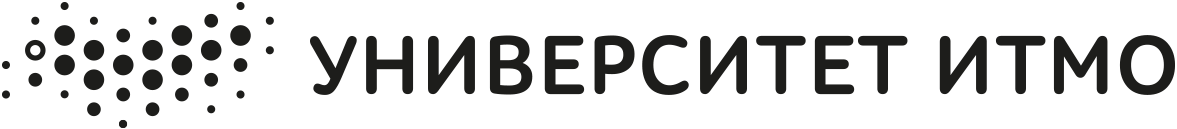
\includegraphics[width=7cm, right]{images/cover/logo_bw.png}
\end{figure}

\noindent\large{\textbf{Университет ИТМО} – национальный исследовательский университет, ведущий вуз России в области информационных, фотонных и биохимических технологий. Альма-матер победителей международных соревнований по программированию – ICPC (единственный в мире семикратный чемпион), Google Code Jam, Facebook Hacker Cup, Яндекс.Алгоритм, Russian Code Cup, Topcoder Open и др. Приоритетные направления: IT, фотоника, робототехника, квантовые коммуникации, трансляционная медицина, Life Sciences, Art\&Science, Science Communication. Входит в ТОП-100 по направлению «Автоматизация и управление» Шанхайского предметного рейтинга (ARWU) и занимает 74 место в мире в британском предметном рейтинге QS по компьютерным наукам (Computer Science and Information Systems). С 2013 по 2020 гг. – лидер Проекта 5-100.} \\ [1ex]

\noindent\large{\copyright \! Университет ИТМО, 2025 \\ 
\copyright \! Новосёлов С.А., Лаврентьева Г.М., Волохов В.А., Матвеев Ю.Н., 2025 \\
\copyright \! Волохов В.А., оформление, 2025}

\end{document}
